\begin{frame}
    \frametitle{The FEniCS challenge!}
    The inflow boundary lies at $x = -0.2$ and the outflow boundary at
    $x=2.0$.
    Compute the flow on the time interval $[0,8]$ with time-step $dt =
    0.001$. Test your implementation first for a larger time-step $dt =
    0.01$ and the same channel problem but with the cylinder removed.
    If everything goes fine you should get something like
    \begin{center}
        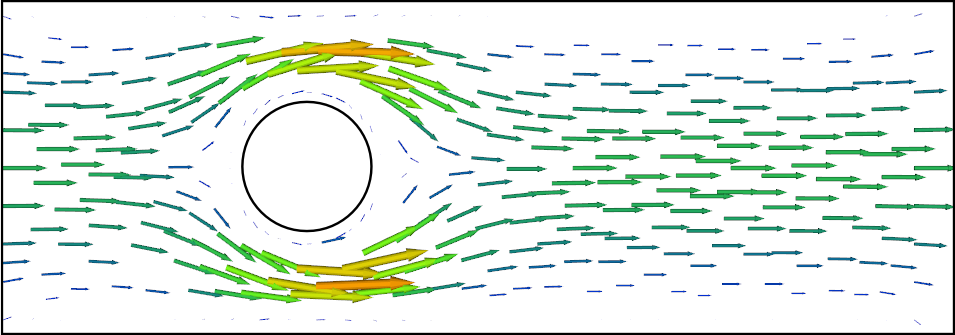
\includegraphics[width=1.0\textwidth]{png/flow_around_cylinder.png}
    \end{center}
    \begin{center}
        {\large Happy coding}!
    \end{center}
    \reference{Sch\"afer/Turek}
              {Benchmark Computations of Laminar Flow Around a
              Cylinder}
              {1996}
\end{frame}
